\capitulo{5}{Aspectos relevantes del desarrollo del proyecto}



\section{Experimentación}

\subsection{Algoritmos de aprendizaje semisupervisado}

\subsubsection{\textit{Co-Forest}}

Para evaluar la calidad del método, se han realizado distintos experimentos con los \textit{dataset} incluídos en la librería \textit{SKlearn} dedicados a la clasificación. Estos son los mostrados en la tabla~\ref{tabla_datasets_sklearn}. El parámetro $n$ representa el número de instancias que contiene un determinado conjunto de datos, mientras que el parámetro $m$ muestra el número de atributos que contiene cada una de esas instancias.

\begin{table}
	\small
	\begin{centering}
		
		\begin{tabular}{@{}p{4em} p{20em} r r r @{}}
			\toprule
			\textbf{Nombre} & \textbf{Descripción} & \textbf{Clases} & $n$ & $m$\\ 
			\midrule
			
			Iris & Conjunto de instancias pertenecientes a diferentes tipos de plantas de la especie Iris. & 3 & 150 & 4 \\\\
			Dígitos & Conjunto de instancias que representan una imagen de 8x8 perteneciente a un dígito. & 10 & 1797 & 64 \\\\
			Vino & Conjunto de instancias pertenecientes tres clases de vino con sus parámetros estimados mediante análisis químico & 3 & 178 & 13 \\\\
			Cáncer de Mama & Conjunto de instancias que representan parámetros de distintas mujeres que pueden padecer o no cáncer (clasificación binaria). & 2 & 569 & 30 \\
		\end{tabular}
		
	\end{centering}
	\caption{Descripción de los \textit{datasets} utilizados para probar el \textit{co-forest}.}
	\label{tabla_datasets_sklearn}	
\end{table}


Se han realizado diferentes experimentos: algunos relacionados con la fase de entrenamiento y otros con el algoritmo una vez finalizado.

\paragraph{Fase de entrenamiento}

Como se ha desarrollado en los conceptos teóricos, la fase de entrenamiento en el \textit{co-forest} es iterativa, y finaliza cuando ningún árbol recibe nuevas pseudo-etiquetas que puedan cambiar su comportamiento (en la fase de re-entrenamiento).

Se ha querido estudiar la evolución de la precisión del algoritmo durante la fase de entrenamiento para los cuatro conjuntos de datos definidos en la tabla~\ref{tabla_datasets_sklearn}. Para ello, se ha realizado una gráfica comprobando cómo evoluciona la precisión del algoritmo en función de la iteración en la que se encuentre.

Para garantizar que los resultados obtenidos no son producto de una partición concreta de los datos, se ha realizado validación cruzada (con 10 particiones). Por lo tanto, el porcentaje de datos utilizados para el entrenamiento es el $90\%$ del total. Los datos de entrenamiento, a su vez, se dividen en etiquetados y no etiquetados. En este caso, el 20\% representa los datos etiquetados, y el 80\% los no etiquetados, como se puede observar en la imagen~\ref{5_entrenamiento_particiones}. Se han utilizado 20 árboles.

\begin{figure}[h]
	\caption{Gráfica que representa la distribución de los datos.}
	\centering
	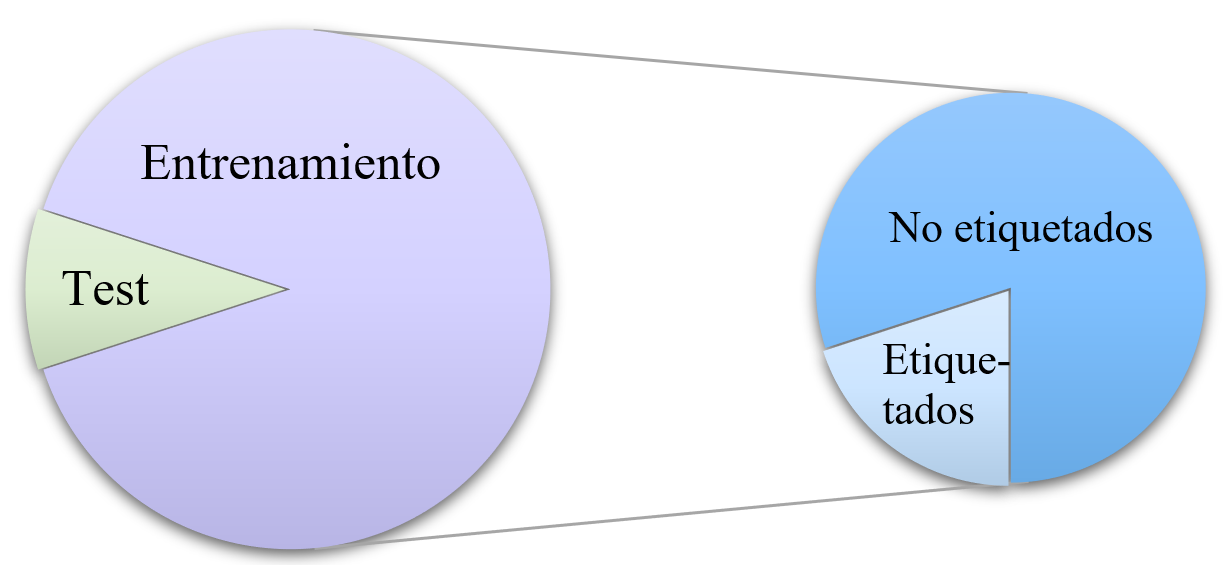
\includegraphics[width=\textwidth]{../img/memoria/5_entrenamiento_particiones}
	\label{5_entrenamiento_particiones}
\end{figure}


 La precisión media obtenida se puede ver representada en la gráfica~\ref{5_coforest_precision-iteraciones}. Es destacable que, dependiendo de los datos que se utilicen para entrenar el \textit{co-forest}, puede variar el número de iteraciones que se necesiten (incluso dentro de un mismo \textit{dataset}). Por ello, siempre se representa el número máximo de iteraciones realizadas, y para no deformar la media, se ha considerado que el valor de las iteraciones inexistentes es el mismo que el valor obtenido en la última iteración (ya que si, el algoritmo siguiese, el resultado devuelto sería igual debido a que no se re-entrenaría ningún árbol).

\begin{figure}[h]
	\caption{Gráfica que representa la precisión del modelo en función de la iteración en la que se encuentre.}
	\centering
	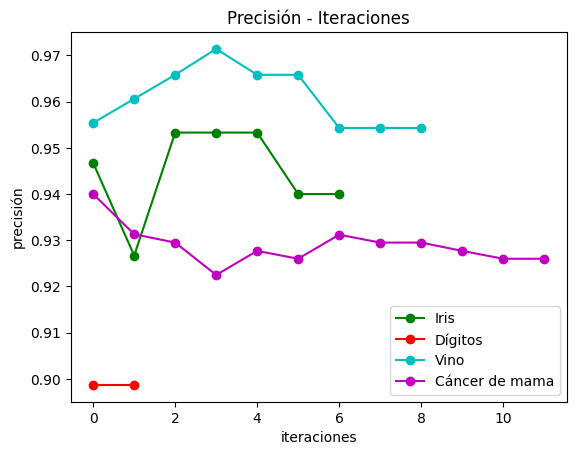
\includegraphics[width=\textwidth]{../img/memoria/5_coforest_precision-iteraciones}
	\label{5_coforest_precision-iteraciones}
\end{figure}


Como se puede comprobar, en general los resultados obtenidos no son satisfactorios debido a que la precisión alcanzada en la última iteración es inferior a la obtenida en la iteración $0$ (cuando todavía no se ha realizado entrenamiento semi-supervisado y se cuenta con un \textit{random forest} normal). Sin embargo, sí se puede observar como en general, en las iteraciones centrales, la precisión inicial es mejorada.

Si se observa con más detenimiento cada conjunto de datos individualmente (gráfica~\ref{5_coforest_precision-iteraciones_individual}), se puede observar que la desviación típica varía considerablemente, por lo que se puede deducir que el modelo podría llegar a ser utilizable si el conjunto de entrenamiento es el adecuado.

\begin{figure}[h]
	\caption{Gráfica que representa, para cada conjunto de datos, la precisión media del modelo en función de la iteración en la que se encuentre junto con la desviación típica para 10 experimentos.}
	\centering
	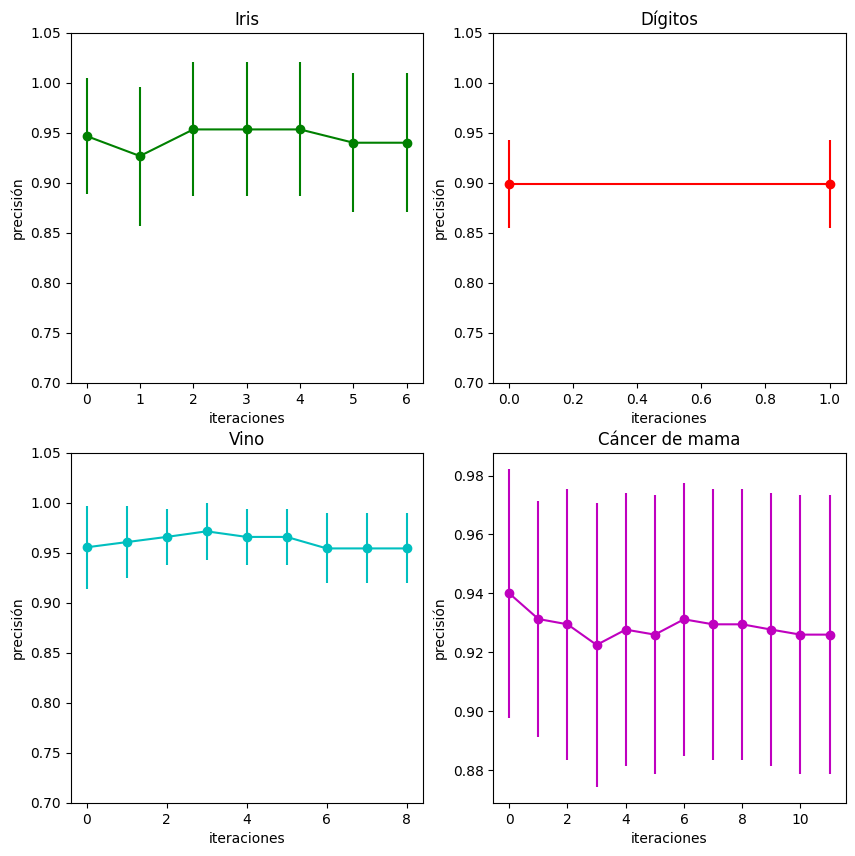
\includegraphics[width=\textwidth]{../img/memoria/5_coforest_precision-iteraciones_individual}
	\label{5_coforest_precision-iteraciones_individual}
\end{figure}


Además, también se ha querido evaluar cómo varía el tiempo de entrenamiento en función del número de instancias utilizadas. Para ello, se ha trabajado con el \textit{dataset} que contiene un mayor número de datos, y los resultados obtenidos se pueden observar en la gráfica~\ref{5_coforest_tiempo-instancias}. Como se puede observar, sigue un crecimiento aproximadamente lineal. La velocidad, en este caso, es alta, pero cabe recordar que depende en gran medida del número de árboles utilizados y de las iteraciones que estos realicen (en este caso, 2).

\begin{figure}[h]
	\caption{Gráfica que representa la evolución del tiempo de entrenamiento en función del número de instancias utilizadas.}
	\centering
	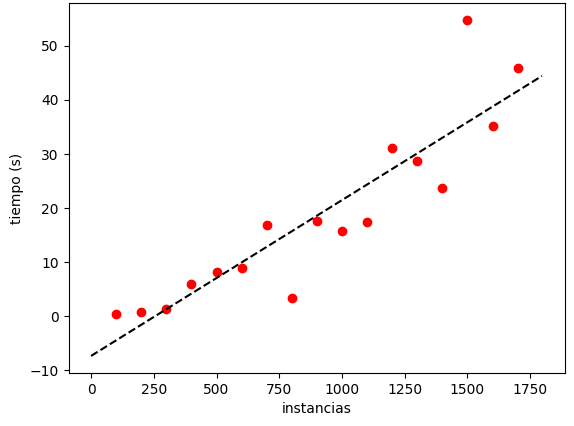
\includegraphics[width=\textwidth]{../img/memoria/5_coforest_tiempo-instancias}
	\label{5_coforest_tiempo-instancias}
\end{figure}
\par


\paragraph{Comportamiento general}

En este apartado de la experimentación, se ha querido evaluar cómo se comporta el \textit{co-forest} en función del porcentaje de datos que se utilice para el entrenamiento. Nuevamente, se han utilizado 20 árboles, y la división del conjunto de datos de entrenamiento se ha mantenido: 20\% etiquetados y 80\% no etiquetados.

Como se puede comprobar en la gráfica~\ref{5_precision-porcentaje_entrenamiento}, se sigue el comportamiento esperado, y por lo general a más instancias utilizadas para entrenar el modelo, mejor comportamiento desarrolla. Nuevamente, recalcar que el resultado obtenido es la media de 10 experimentos realizados.

\begin{figure}[h]
	\caption{Gráfica que representa la precisión media del modelo en función del porcentaje de datos utilizados para el entrenamiento.}
	\centering
	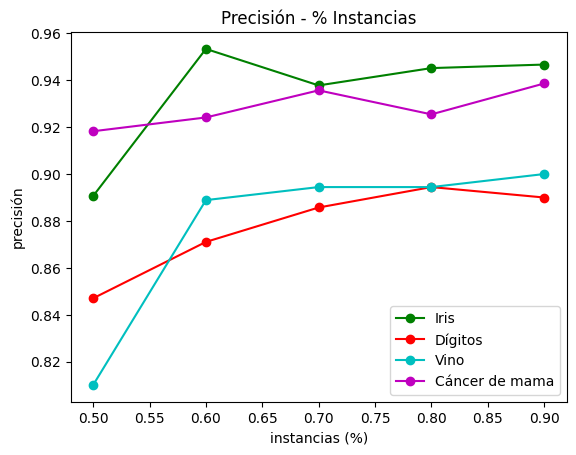
\includegraphics[width=\textwidth]{../img/memoria/5_precision-porcentaje_entrenamiento}
	\label{5_precision-porcentaje_entrenamiento}
\end{figure}
\par

Se representa además, en la gráfica~\ref{5_precision-porcentaje_entrenamiento_individual} la desviación media obtenida en los 10 experimentos para cada conjunto de datos.

\begin{figure}[h]
	\caption{Gráfica que representa, para cada conjunto de datos, la precisión media del modelo y su desviación en función del porcentaje del conjunto utilizado para el entrenamiento.}
	\centering
	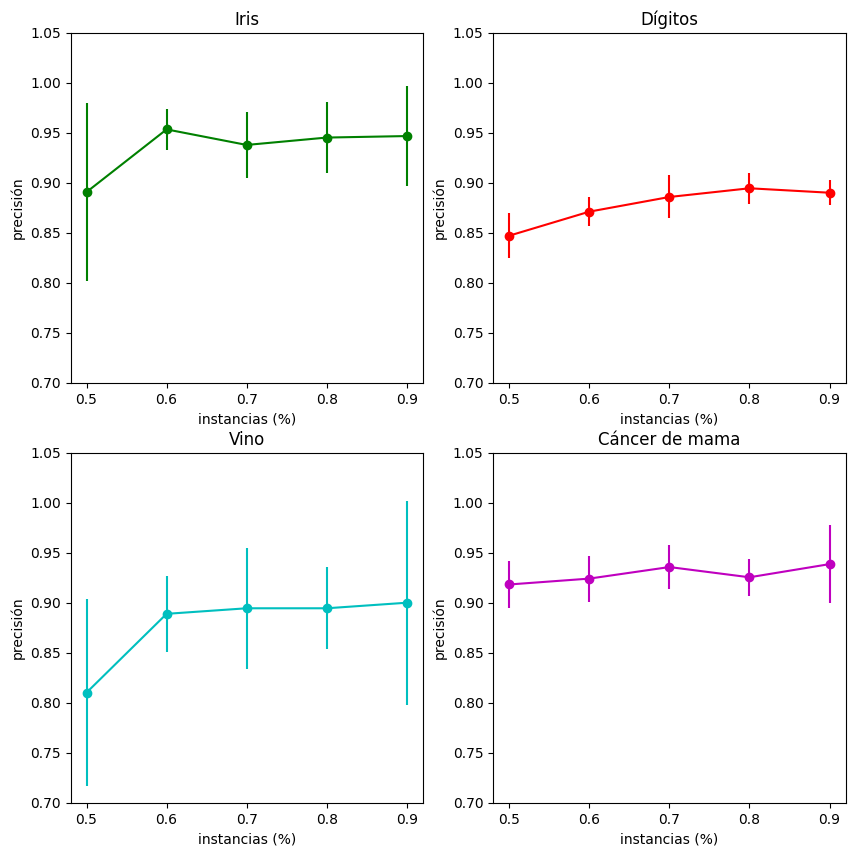
\includegraphics[width=\textwidth]{../img/memoria/5_precision-porcentaje_entrenamiento_individual}
	\label{5_precision-porcentaje_entrenamiento_individual}
\end{figure}
\par
